\documentclass[compress]{beamer}
\usepackage{ifthen,verbatim}

\newcommand{\isnote}{}
\xdefinecolor{lightyellow}{rgb}{1.,1.,0.25}
\xdefinecolor{darkblue}{rgb}{0.1,0.1,0.7}

%% Uncomment this to get annotations
%% \def\notes{\addtocounter{page}{-1}
%%            \renewcommand{\isnote}{*}
%% 	   \beamertemplateshadingbackground{lightyellow}{white}
%%            \begin{frame}
%%            \frametitle{Notes for the previous page (page \insertpagenumber)}
%%            \itemize}
%% \def\endnotes{\enditemize
%% 	      \end{frame}
%%               \beamertemplateshadingbackground{white}{white}
%%               \renewcommand{\isnote}{}}

%% Uncomment this to not get annotations
\def\notes{\comment}
\def\endnotes{\endcomment}

\setbeamertemplate{navigation symbols}{}
\setbeamertemplate{headline}{\mbox{ } \hfill
\begin{minipage}{5.5 cm}
\vspace{-0.75 cm} \small
\end{minipage} \hfill
\begin{minipage}{4.5 cm}
\vspace{-0.75 cm} \small
\begin{flushright}
\ifthenelse{\equal{\insertpagenumber}{1}}{}{Jim Pivarski \hspace{0.2 cm} \insertpagenumber\isnote/\pageref{numpages}}
\end{flushright}
\end{minipage}\mbox{\hspace{0.2 cm}}\includegraphics[height=1 cm]{../cmslogo} \hspace{0.1 cm} \includegraphics[height=1 cm]{../tamulogo} \hspace{0.01 cm} \vspace{-1.05 cm}}

\begin{document}
\begin{frame}
\vfill
\begin{center}
\textcolor{darkblue}{\Large State of Muon Alignment \\ \vspace{0.2 cm} and What Needs to be Done}

\vfill
\begin{columns}
\column{0.3\linewidth}
\begin{center}
\large
\textcolor{darkblue}{Jim Pivarski}
\end{center}
\end{columns}

\begin{columns}
\column{0.3\linewidth}
\begin{center}
\scriptsize
{\it Texas A\&M University}
\end{center}
\end{columns}

\vfill
10 November, 2009

\end{center}
\end{frame}

%% \begin{notes}
%% \item This is the annotated version of my talk.
%% \item If you want the version that I am presenting, download the one
%% labeled ``slides'' on Indico (or just ignore these yellow pages).
%% \item The annotated version is provided for extra detail and a written
%% record of comments that I intend to make orally.
%% \item Yellow notes refer to the content on the {\it previous} page.
%% \item All other slides are identical for the two versions.
%% \end{notes}

\small

\begin{frame}
\frametitle{State of A\&M muon alignment}
\textcolor{darkblue}{\large The good news}

\begin{itemize}
\item Our Reference-Target procedure seems to be recognized as the {\it de facto} track-based muon alignment method for CMS
\item Hardware alignment system is being diagnosed via comparisons with our track-based data (rather than the other way around)
\item Our CSC-Overlaps procedure has been conclusively demonstrated with last year's beam-halo, and has been successfully tested with this year's Monte Carlo (new)
\item The 2008 beam-halo/CRAFT paper (09-016) has been accepted by the collaboration (this is our only documentation so far)
\item Our Tracker-To-Ring alignment has been tested in CRAFT-2009 (CSC-Overlaps $+$ Tracker-To-Ring is a complete endcap alignment)
\end{itemize}

\textcolor{darkblue}{\large What comes next}
\begin{itemize}
\item Large quantities of beam-halo: must align all CSCs with beam-halo (CSC-Overlaps) and cosmic rays (Tracker-To-Ring)
\item First collisions: must align all DTs with low-$p_T$ muons \mbox{(Reference-Target)\hspace{-1 cm}}
\end{itemize}
\end{frame}

\begin{frame}
\frametitle{Problems and open questions}
\framesubtitle{In order of importance}

\begin{itemize}
\item Both DT and CSC alignments exhibit dependence on \mbox{track $p_T$ (hard)\hspace{-1 cm}}
\begin{itemize}\setlength{\itemsep}{0.1 cm}
\item cannot apply interim solution, a $p_T > 100$~GeV cut, with collisions (cosmics $\sim {p_T}^{-2.7}$, collisions $\sim \exp(-{p_T})$)
\item DT problem: probably a global distortion of the tracker
\item CSC problem: $p_T$ dependence alternates sign \mbox{between chambers\hspace{-1 cm}}
\end{itemize}

\item We don't know how alignment resolution depends on $\int \mathcal{L} \, dt$ (easy)

\item findQualityFiles.py doesn't seem to work (?)

\item Need to complete documentation

\item Will eventually need the following new features:
\begin{itemize}\setlength{\itemsep}{0.1 cm}
\item alignment of ME1/1, 1/4 CSCs in rigid 2-chamber groups (physically the same chambers, independent units in software)
\item radial alignment of DTs in rigid 5-chamber groups \\ (if pre-alignment is guaranteed by hardware system)
\item ability to align radial positions of CSCs \mbox{(a very different project)\hspace{-1 cm}}
\item ability to align internal layers, especially in CSCs
\end{itemize}
\end{itemize}
\end{frame}

\begin{frame}
\frametitle{DT $p_T$ dependence}

\begin{itemize}
\item Quick study: select a single DT layer (wheel, station, sector,
  layer: 0, 1, 10, 2) to avoid any dependence on internal muon misalignment
\item Plot ``unbiased residuals'' as a function of $q/p_T$ (curvature)
\item Misalignment of the DT layer would be constant in $q/p_T$,
  magnetic field or material budget errors would be antisymmetric in
  $q/p_T$
\end{itemize}

\begin{columns}
\column{0.6\linewidth}
\includegraphics[height=0.48\linewidth, angle=90]{residx-qoverpt_real.pdf}
\includegraphics[height=0.48\linewidth, angle=90]{residx-qoverpt_ideal.pdf}

\includegraphics[height=0.48\linewidth, angle=90]{residx-qoverpt_layerRotation.pdf}
\includegraphics[height=0.48\linewidth, angle=90]{residx-qoverpt_sagitta.pdf}

\column{0.3\linewidth}
\mbox{\hspace{-0.75 cm}\begin{minipage}{1.2\linewidth}
\begin{itemize}
\item Top-left: real data, CRAFT-2009 in 3\_2\_7 with the latest tracker alignment
\item Others: Monte Carlo with different tracker geometries
\item blues: \mbox{2-D distribution\hspace{-1 cm}} \\ of residuals vs.~$q/p_T$
\item black points: profile \mbox{(vertical mean by bin)\hspace{-1 cm}}
\end{itemize}
\end{minipage}}
\end{columns}
\end{frame}

\begin{frame}
\frametitle{DT residual vs.~$\phi$ and $q/p_T$}

\begin{itemize}
\item 2-D profiles: color scale is average residual (mm) in each 2-D bin
\item None of the 9 example tracker distortions has exactly the same shape as data
\item This is a tracker alignment issue; shown in \mbox{tracker alignment meeting\hspace{-1 cm}}
\end{itemize}

\begin{columns}
\column{0.4\linewidth}
\includegraphics[height=\linewidth, angle=90]{residx-phi-qoverpt_real.pdf}

\column{0.6\linewidth}
\includegraphics[height=0.32\linewidth, angle=90]{residx-phi-qoverpt_radial.pdf}
\includegraphics[height=0.32\linewidth, angle=90]{residx-phi-qoverpt_telescope.pdf}
\includegraphics[height=0.32\linewidth, angle=90]{residx-phi-qoverpt_layerRotation.pdf}

\includegraphics[height=0.32\linewidth, angle=90]{residx-phi-qoverpt_bowing.pdf}
\includegraphics[height=0.32\linewidth, angle=90]{residx-phi-qoverpt_zExpansion.pdf}
\includegraphics[height=0.32\linewidth, angle=90]{residx-phi-qoverpt_twist.pdf}

\includegraphics[height=0.32\linewidth, angle=90]{residx-phi-qoverpt_elliptical.pdf}
\includegraphics[height=0.32\linewidth, angle=90]{residx-phi-qoverpt_skew.pdf}
\includegraphics[height=0.32\linewidth, angle=90]{residx-phi-qoverpt_sagitta.pdf}
\end{columns}
\end{frame}

\begin{frame}
\frametitle{CSC $p_T$ dependence}
\begin{columns}
\column{0.65\linewidth}
\includegraphics[width=\linewidth]{wasitthepropagator_before.png}

\includegraphics[width=\linewidth]{wasitthepropagator_after.png}
\column{0.35\linewidth}
\begin{itemize}
\item Alternation of residuals from one chamber to the next

\item Non-physical: the chambers wouldn't move like that

\item $p_T > 40$~GeV cut $\to$ $p_T > 100$~GeV suppresses the effect

\item Not observed in RecHits (overlaps)

\item Unclear what the effect is (not $\vec{B}(\vec{x})$, as that wouldn't alternate)
\end{itemize}
\end{columns}
\end{frame}

\begin{frame}
\frametitle{Who should work on this?}
\begin{itemize}\setlength{\itemsep}{0.5 cm}
\item DT $p_T$ dependence: likely a tracker alignment issue, may be
  solved by tracker alignment with early collisions, resonances, etc.
\begin{itemize}
\item I'm trying to get someone to use the method I presented to
  diagnose the tracker
\item Not for our group (tracker alignment is not our scope)
\end{itemize}
\item CSC $p_T$ dependence: I might be able to figure something out by
  comparing overlapping CSCs (beam-halo) with tracks from the tracker
  (cosmics)
\begin{itemize}
\item very open-ended problem, because symptoms don't make sense
\item CSC-DPG is aware of it, I'm encouraging others to look at it
\end{itemize}
\end{itemize}
\end{frame}

\begin{frame}
\frametitle{Dependence on $\int \mathcal{L} \, dt$}
\begin{itemize}\setlength{\itemsep}{0.1 cm}
\item We're starting to get questions about when we'll be able to
  provide a first alignment of all chambers (cosmic ray alignment only
  covers top and bottom, where the cosmic rays are)
\item Usual answer of 20--50~pb$^{-1}$ is no longer acceptable
  (50~pb$^{-1}$ is no longer considered a small amount of data)
\item Natural conclusion of ``October Exercise'' study:
\begin{itemize}
\item split sample into non-overlapping samples: 5, 10, 20, 50~pb$^{-1}$ or something
\item run procedure (correctly) on each
\item quote results
\end{itemize}
\end{itemize}

\vfill
\hspace{-0.83 cm} \textcolor{darkblue}{\Large findQualityFiles.py not working}
\begin{itemize}\setlength{\itemsep}{0.1 cm}
\item I tried to use it to select within a run range, it selected zero runs
\item I was in a hurry, so I did it by hand
\item It needs to be made robust, at least in a stand-alone CMSSW directory
\end{itemize}
\end{frame}

\begin{frame}
\frametitle{Documentation}
\begin{itemize}
\item We're building up new a tree (starting summer 2008) under

{\tt \scriptsize https://twiki.cern.ch/twiki/bin/view/CMS/SWGuideMuonAlignment}

\item findQualityFiles.py should become a separate page, not in the flow of the Reference-Target documentation
\end{itemize}

\vfill
\hspace{-0.83 cm} \textcolor{darkblue}{\Large Who should work on this?}
\begin{itemize}
\item Clearly, I have to write the first draft of each topic

\item But it would be very helpful if you could expand, polish, or
  otherwise make it more useable as you try to use it
\begin{itemize}
\item our e-mail discussions have made SWGuideMuonAlignReferenceTarget out-of-date
\end{itemize}
\end{itemize}
\end{frame}

\begin{frame}
\frametitle{New features 1}

\vspace{-0.5 cm}
\hspace{3 cm} 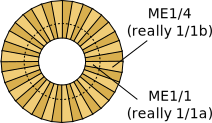
\includegraphics[width=0.25\linewidth]{me11.pdf}

\begin{itemize}
\item CMSSW makes a distinction between the 1/1a half and the 1/1b half of ME1/1 chambers (models them as separate chambers)
\item They are physically part of the same frame; we should treat them as rigid bodies for alignment
\item I implemented this in Reference-Target, but it seemed to not be working, so it is off by default
\item It has not been implemented in CSC-Overlaps, but it needs to be
\end{itemize}

\vfill
\hspace{-0.83 cm} \textcolor{darkblue}{\Large Who should work on this?}
\begin{itemize}
\item I should just find and fix the bug
\item But I may ask for your help in testing (i.e.\ run a simulated collisions alignment to check that it was handled properly)
\item I'll need to copy the implementation into CSC-Overlaps
\end{itemize}
\end{frame}

\begin{frame}
\frametitle{New features 2: DT radial}

\begin{columns}
\column{0.5\linewidth}
\includegraphics[width=\linewidth]{dt_coordinates.pdf}

\column{0.5\linewidth}
\begin{itemize}
\item Radial (local $z$) alignment of DTs is only weakly determined by tracks
\begin{itemize}
\item $\delta_z$ correction is effectively the slope of $\Delta x$
  residuals versus $\frac{dx}{dz}$ entrance angle or $\Delta y$
  residuals versus $\frac{dy}{dz}$ entrance angle
\item distributions of entrance angles are narrow, limiting the precision of the slope
\end{itemize}
\end{itemize}
\end{columns}

\begin{itemize}
\item $\Delta x / \frac{dx}{dz}$ and $\Delta y / \frac{dy}{dz}$ can be antisymmetric with $q/p_T$, just like magnetic field and material budget errors: normal trick doesn't work
\item If we could assume that 5-chamber groups spanning all 5 wheels
  are at {\it the same} $z$ position, we would gain a much broader
  expanse of $\frac{dy}{dz}$ by aligning them together as rigid bodies
  (in $z$ only; for the other parameters, we do normal single-chamber alignment)
\end{itemize}
\end{frame}

\begin{frame}
\frametitle{New features 2: DT radial}
\includegraphics[width=0.5\linewidth]{zfits_normal.pdf}\includegraphics[width=0.5\linewidth]{zfits_alternative.pdf}

\begin{itemize}
\item Hacked together a test, and it does seem that the hardware alignment provides relatively consistent $z$ positions
\end{itemize}

\begin{columns}
\column{0.7\linewidth}
\includegraphics[height=\linewidth, angle=90]{zfit_1_05.pdf}

\column{0.3\linewidth}
\includegraphics[width=\linewidth]{zfits_chi2.pdf}
\end{columns}
\end{frame}

\begin{frame}
\frametitle{New features 3: CSC radial}

\begin{itemize}
\item CSC wire measurements are not good for alignment: huge granularity (several cm) yields non-bell-curve residuals
\item Both Reference-Target and CSC-Overlaps use strip data only; very little sensitivity to radial positions (local $y$)
\item Can identify radial position by observing location of inefficiencies at regular intervals on the chambers, instead of residuals
\item This would be a very different kind of project, separate framework
\end{itemize}

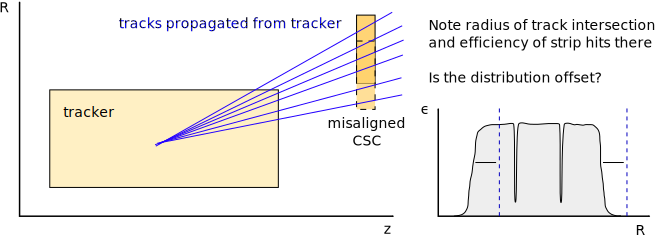
\includegraphics[width=\linewidth]{way_to_find_radial_misalignment.pdf}
\end{frame}

\begin{frame}
\frametitle{New features 4: layer alignment}

\begin{itemize}
\item Track-based layer alignment has the best resolution when using only local linear segments
\item Our chamber geometries ($N$ parallel layers) have serious weak modes when doing so (especially shear of the chamber and all segments)
\item Using overlapping tracks in the CSCs only turns this into a ring-wide problem
\item One could develop a hybrid procedure where the slope of the
  segment is derived from a track propagated from the tracker and the
  intercept is from locally-fitted data
\begin{itemize}
\item track angles propagated from the tracker are unambiguous
\item segment positions from a local fit are precise
\end{itemize}
\item We have stayed out of DT layer alignment, and should continue to do so for the foreseeable future
\item CSC layers appear to be well aligned already (in ME$-$2/1, $-$3/1)
\item Oleg's hardware alignment of CSC layers has the same weak modes (by coincidence)
\end{itemize}
\end{frame}

%% \begin{frame}
%% \frametitle{Outline}
%% \begin{itemize}\setlength{\itemsep}{0.75 cm}
%% \item 
%% \end{itemize}
%% %% \hspace{-0.83 cm} \textcolor{darkblue}{\Large Outline2}
%% \end{frame}

%% \section*{First section}
%% \begin{frame}
%% \begin{center}
%% \Huge \textcolor{blue}{First section}
%% \end{center}
%% \end{frame}

\begin{frame}
\frametitle{Conclusions}
\begin{itemize}
\item Lots to do!
\item We should figure out short/long-term goals and who does what in this meeting
\end{itemize}
\label{numpages}
\end{frame}

\end{document}
